%
% 2010.01.24 情報システム工学科対応
% 2018.01.05 電子・情報工学科対応
%
\documentclass[10pt]{tpu-abst-utf}
\usepackage[dvipdfmx]{graphicx}
\usepackage{listings}
\lstset{
basicstyle={\small},% 
identifierstyle={\small},% 
commentstyle={\small\ttfamily \color[rgb]{0,0,0}},% 
keywordstyle={\small\bfseries \color[rgb]{0,0,1}},% 
ndkeywordstyle={\small},% 
stringstyle={\small\ttfamily}, 
frame={tb}, 
breaklines=true, 
columns=[l]{fullflexible},% 
numbers=left,% 
xrightmargin=0zw,% 
xleftmargin=3zw,% 
numberstyle={\scriptsize},% 
stepnumber=1, 
numbersep=1zw,% 
morecomment=[l]{//}% 
}
%
% ここでタイトルの設定をします
%
% 自分の名前
\author{佐原 優衣}
%
% 学籍番号
\gakuban{1515024}
%
% 研究室の番号
\kouzanum{2}
% 1 情報基盤工学講座 
% 2 情報システム工学講座 
% 3 集積機能デバイス工学講座 
% 4 電子通信システム工学講座 
%
%
% 指導教員名: 
% \kouzaname{ななし} % これはコメントアウトする
% \kouzaname{太田} % 
% \kouzaname{奥原} % 
% \kouzaname{西田} % 
% \kouzaname{榊原} % 
\kouzaname{中村(正)} % 
% \kouzaname{松本(三)} % 
% \kouzaname{唐山} % 
% \kouzaname{鳥山} % 
% \kouzaname{岩本} % 
% \kouzaname{安宅} % 
% \kouzaname{中田} % 
% \kouzaname{浦島} % 
% \kouzaname{松田(敏)} % 
% \kouzaname{岩田} % 
% \kouzaname{松田(弘)} % 
% \kouzaname{石坂} % 
% \kouzaname{三宅} % 
% \kouzaname{小林(香)} % 
% \kouzaname{小島} % 
%
% 発表番号
\happyou{18}
%
% タイトル
\title{UPPAALを用いた自動運転車の\\群制御アルゴリズムのモデル化と検証}
%
%----- begin document
%
\begin{document}
%
\maketitle
%
%----- your abstract, please
%
\section{研究背景と目的}
%1--
従来より,自動運転技術は発達し続けている。道路交通は自動運転車のみで構成される都市空間を考える。多数の自動運転車が発生する都市空間では,道路上車両密度が高くなるため,様々な問題が発生する可能性がある。したがって自動運転車群に対する効率的な群制御アルゴリズムが必要となる。
	
しかし,効率的なアルゴリズムが本当に問題がないかどうか確証がない。そこで本研究では群制御アルゴリズムをモデル化し,その性質を検証する手法を提案する。

モデル検査は,システム上で起こり得る状態を網羅的に調べることにより設計の誤りを発見する自動検証手法の一種である。モデル検査手法は,図\ref{ModelV}に示す様に,システムの振る舞いの設計,および検証したい性質をそれぞれモデル化し,ツールを用いて,システムが性質を満たしているかを調べる。本研究では,時間オートマトンによる時間制約検証が行えるUPPAALを採用する。
	\begin{figure}[htbp]
	\centering
	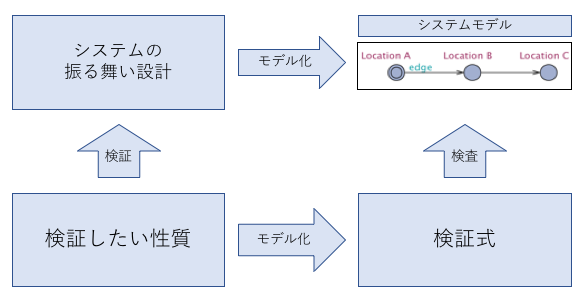
\includegraphics[width=75mm]{ModelVerification.png}
	\caption{モデル検査とは}
	\label{ModelV}
	\end{figure}
%2--
\section{UPPAALを用いたモデル化と検証}
UPPAALを用いて交差点を通過する1台の車両の時間オートマトンを作成する。
%{4台の車両が出発地点から到着地点まで,それぞれ違う方向から一つの交差点に進入し,通過するとする。なお,この交差点には右折レーン,信号がないものとする。平行な向きの車両はお互いに止まることなく通過するが,進行方向が垂直に交差する場合は先に交差点への進入権を獲得した方が先に通過する。そのために交差点への進入権をいつ獲得し,交差点の通過にかかる時間も考慮する。}
この車両は交差点進入前,交差点通過中,通過後の3つの状態に分けられる。交差点の進入前に交差点の使用権を獲得し,通過後に交差点の使用権を返却する。
\begin{figure}[htbp]
\centering
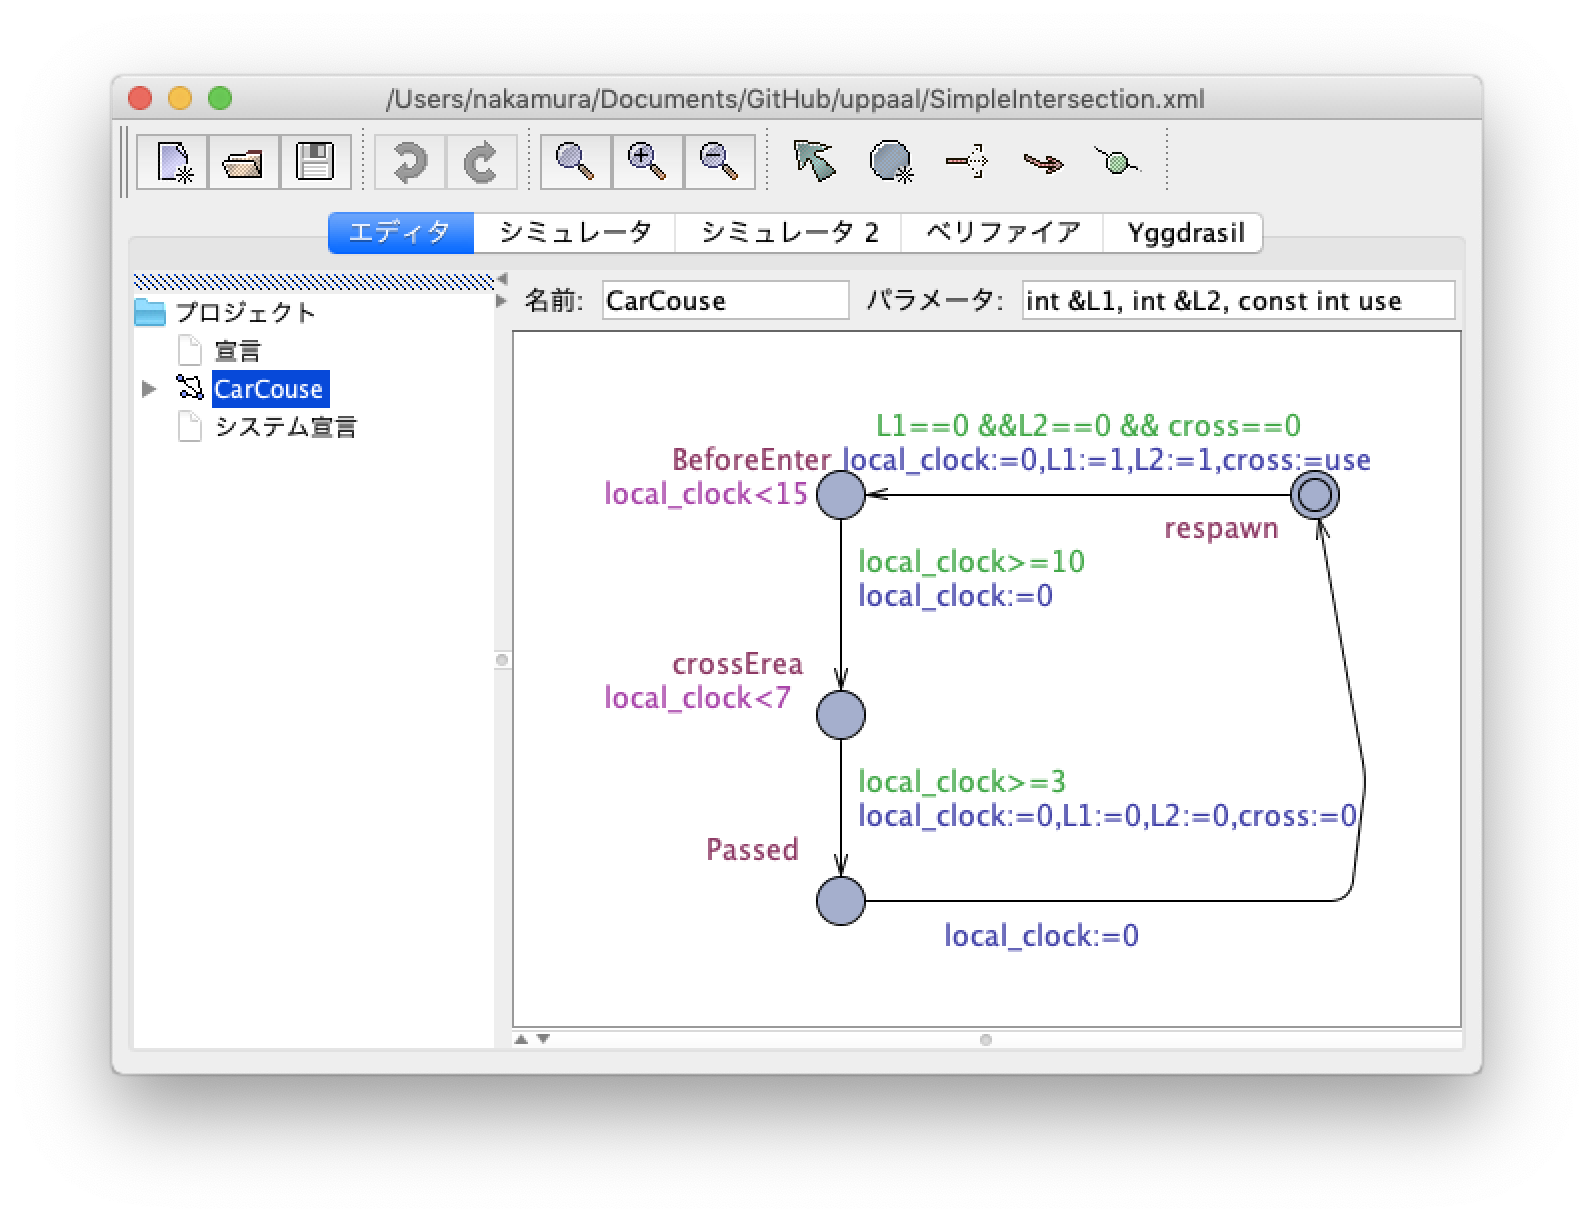
\includegraphics[width=70mm]{Simple.png}
\caption{車両一台の交差点通過モデル}
\label{Simple}
\end{figure}
\section{まとめ}
本研究では,UPPAALを用いた群制御アルゴリズムのモデル化と検証の手法を提案した。単一の交差点においては車両の挙動をモデル化し,通過時間や衝突回避を検証することができた。しかし,都市空間には交差点は複数存在する。したがって,複数の交差点からなるモデルを作成し検証することが今後の課題である。
\begin{thebibliography}{1}
\bibitem{no1}{\small 長谷川哲夫,田原康之,磯部祥尚,UPPAALによる性能モデル検証ーリアルタイムシステムのモデル化と検証ー,(株)近代科学社,2012}
\end{thebibliography}
%
\end{document}
